\section{Functional Flow Diagram}
\label{section_FFD}
The \ac{FFD} shows the functions the system needs to perform during its mission life. The schematic representation can be found in figure \ref{pic_FFD} on page \pageref{pic_FFD}.
\\ \\
The first thing that needs to happen, after being build, is that the satellites are put into their orbits and pointed towards Earth. After that the measurements can start; the emitter sends down laser pulses and notifies the receivers signals are sent. The receivers can adjust their attitude, pick up reflected photons, turn them into an electric signal and inform the computer, which puts the data in a buffer. The data of the receivers can be either transmitted directly to a ground station or first sent to the main satellite (the emitter) and then to the ground. The data on the ground can be split up into data packages, which can be distributed to research institutes and other interested parties. With those data sets, the terrain model can be produced. At the \ac{EOL} of the mission the satellites are decommissioned to make room for other satellites.

\begin{figure}
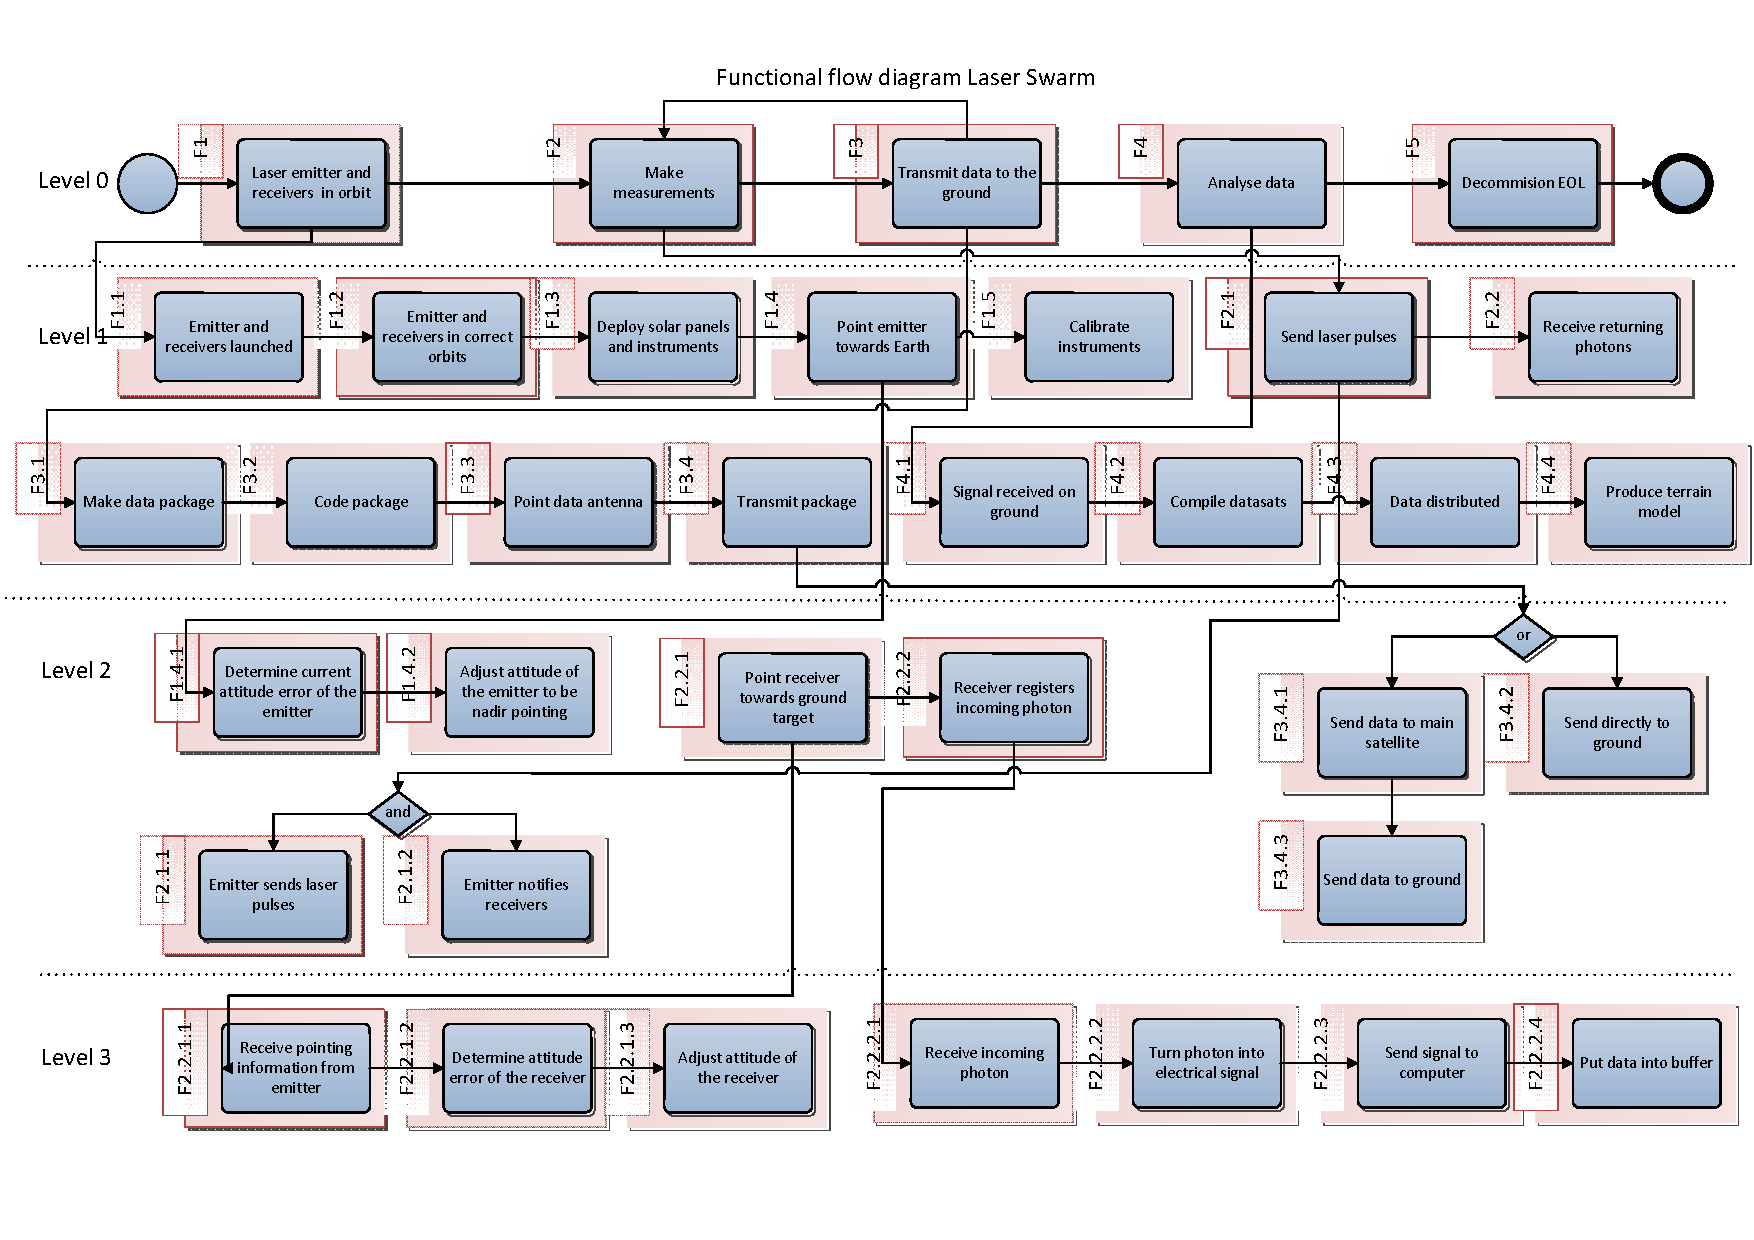
\includegraphics[scale=0.7, angle=90]{chapters/img/pic_FFD.pdf}
\label{pic_FFD}
\caption{Functional flow diagram of the Laser Swarm mission}
\end{figure}

\section{Functional Breakdown Structure}
\label{section_FBS}
The \ac{FBS} shows the functions the system needs to perform broken up in subtasks from other functions. The schematic representation can be found in figure \ref{pic_FBS} on page \pageref{pic_FBS}.
\\ \\
The main function for the system is to be able to produce a terrain model, which is the reason to make the measurements. To be able to produce the terrain model the measurements need to be made, the data needs to be transferred to the ground and the data needs to be analysed. Because the mission needs to be sustainable the satellites are decommissioned at the end of their life, so they will not pose a threat to other satellites in the same orbit.
The making of measurements depends on laser pulses to be send, returning photons to be detected and for the emitter and receivers to be in orbit with the instruments calibrated. For the data to be transmitted to Earth the antenna needs to be pointed to the ground station and the data package has to be transmitted. Data analysis depends on the data to be received on the ground and the distribution between the research institutes.
\\ \\
To have the satellite send out laser pulses the satellite needs to point down (nadir-pointing) and the emitter sends the pulses. The receiving of photons depends on the receiver being pointed at the ground target and the receiver is able to register incoming photons. For the data package to be transmitted, data is put into a buffer, a data package is made, the package is code and either the receiver sends the data to the ground directly or to the main satellite, which in turn forwards it to Earth. When the emitter and receiver are in orbit, the emitter and receivers have been launched and they need to be on the correct orbits. It is important to have the solar panels and instruments to be deployed before they can be calibrated.
\\ \\
Determining the attitude error of the emitter and adjusting the attitude accordingly are required to point the emitter towards Earth. When an incoming photon is received, it is transformed into an electrical signal and the signal is sent to the on-board computer the photon is registered. For the receiver to be pointed at the ground target, the emitter needs to notify the receiver it has sent pulses, the receiver needs to receive the message, the attitude error of the receiver needs to be determined and the attitude should be adapted accordingly. 

\begin{figure}
\begin{center}
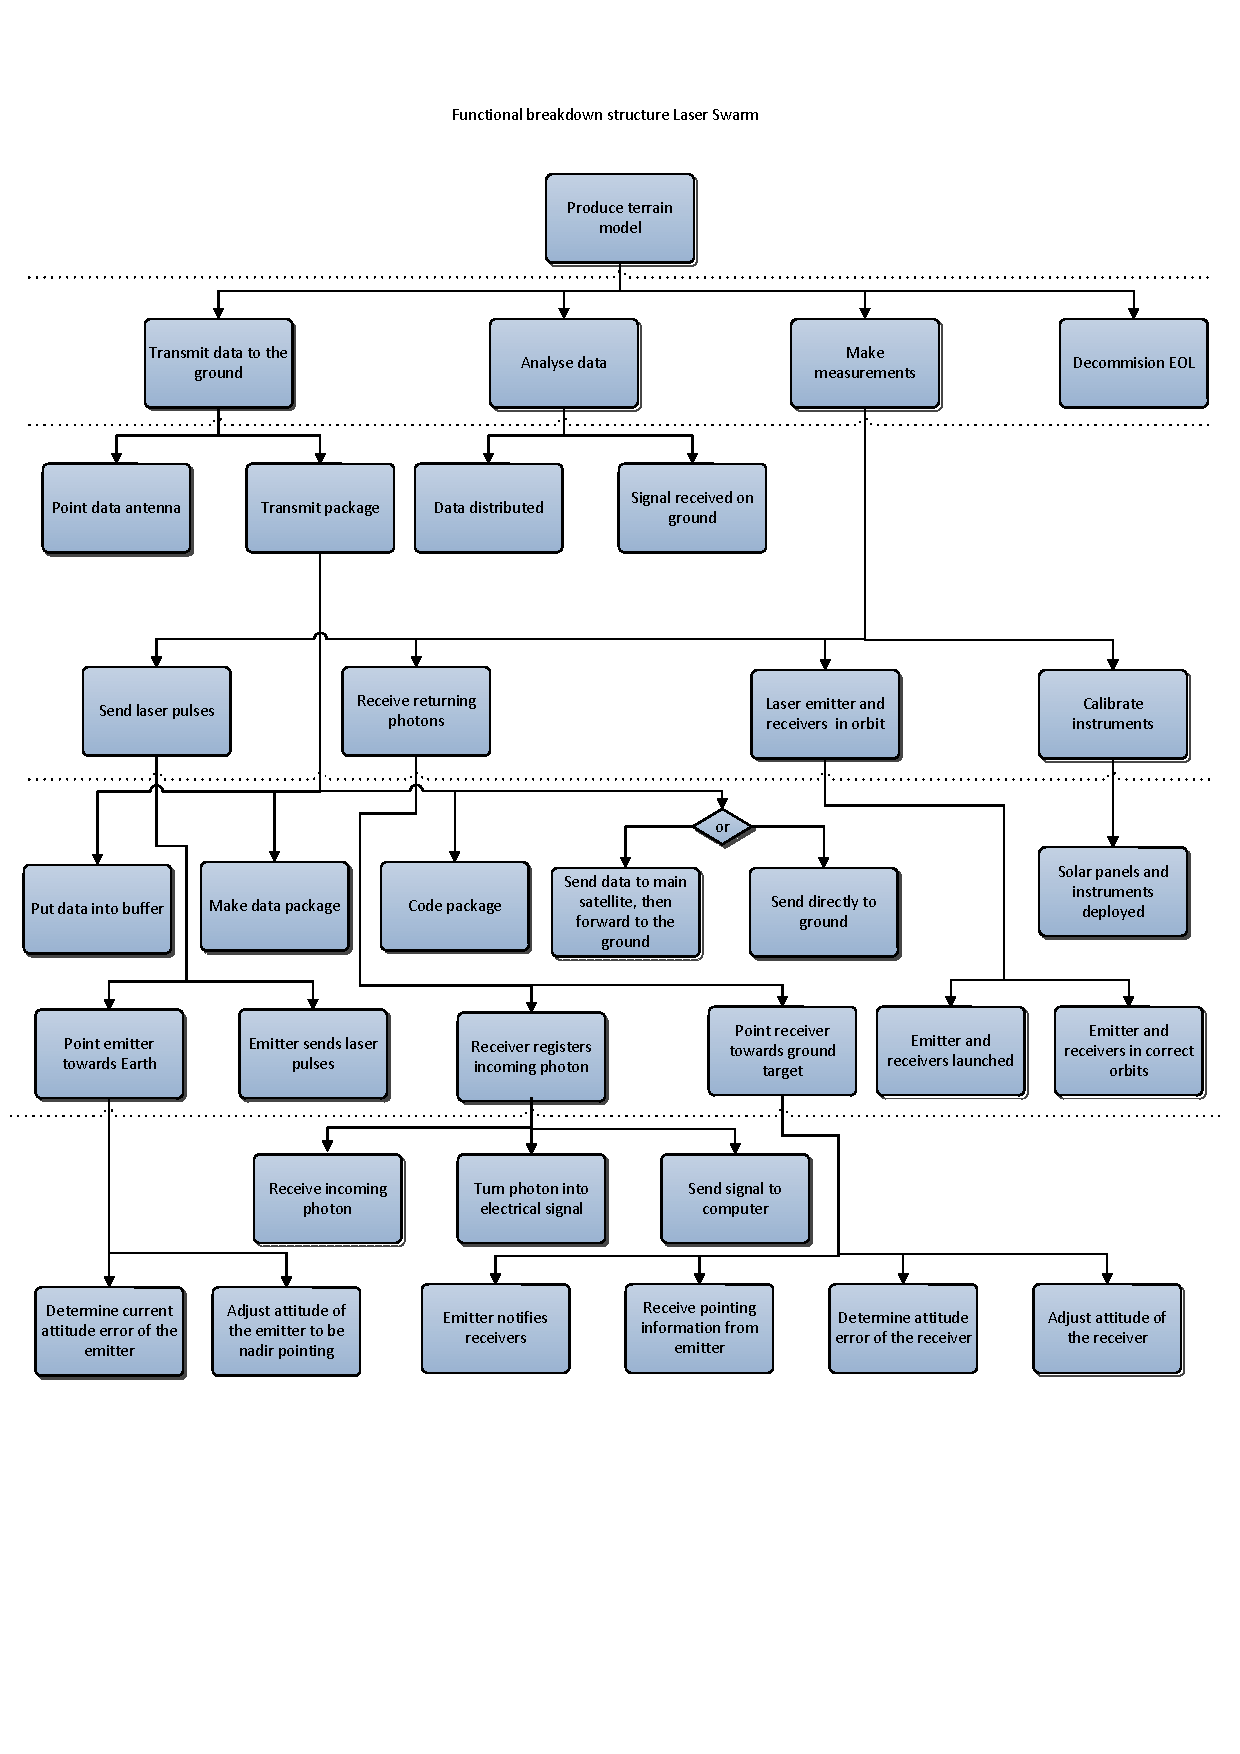
\includegraphics[trim = 0mm 60mm 0mm 0mm, clip, scale=0.7]{chapters/img/pic_FBS.pdf}
\label{pic_FBS}
\caption{Functional breakdown structure of the Laser Swarm mission}
\end{center}
\end{figure}